\chapter{Méthode CDLOD}

  La méthode \textbf{CDLOD}, pour "Continuous Distance-Dependent Level of Detail for Rendering Heightmaps" (Niveau de détail continu dépendant de la distance pour le rendue de carte de hauteur") par Filip Strugar \cite{CDLOD}, 
  est un algorithme qui comme son nom l'indique, se base sur la distance pour l'affichage du niveau de détail 
  (\textbf{LOD}) basé sur une carte de hauteur (\textbf{Heightmaps}).

  De nombreux algorithme se servent de niveaux de détail pour générer leurs terrains.Mais, un des problèmes majeurs auxquels ils se confrontent viens dès lors de la séparation entre deux niveaux de détail voisins.\\
 \begin{wrapfigure}[6]{r}{6cm}
 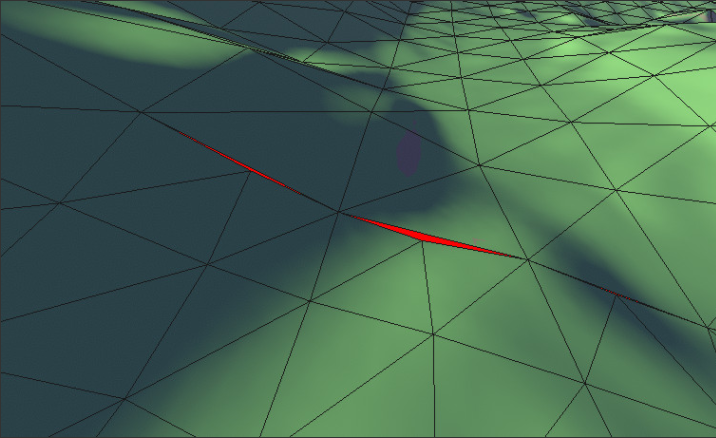
\includegraphics[width=6cm]{img/seams.png}
   \caption[Discontinuité]{Discontinuité\protect\footnotemark}
   \label{fig:seams}
 \end{wrapfigure}
 \footnotetext{Extrait de \url{http://mikejsavage.co.uk/blog/geometry-clipmaps.html}}
 
 \vspace{0.5cm}
 En effet la différence d'élévation entre chaque divisions peuvent provoquer une discontinuité provoquant ainsi une zone vide, 
 comme on peut le voir, par la zone rouge indiqué sur cette image. 
 
 
 \vspace{2cm}
 La méthode utilisé en général pour de palier à cette discontinuité est de rajouter des connexions entre les niveaux affectés. 
 Cette solution a de nombreux inconvénient, en rajoutant des connexions de cette manière, lors du rendue et, lors du parcours du terrain ,ces connexions vont alors apparaître brusquement perturbant ainsi la fluidité. À cela viennent s'ajouter la possibilité d'avoir des connexions multiple superposé et également un coût de rendue supplémentaire en terme de calcul et de mémoire.
 
 L'algorithme CDLOD va notamment ce différencier ici des autres algorithmes par ses "transitions fluides" entre les niveaux de détails par une méthode dites de "\textbf{morphing}" dont nous reparlerons après avoir expliqué l'algorithme plus en détails.
 
 Pour pouvoir correctement expliqué l'algorithme il est tout d'abord nécessaire d'introduire les notions de  \textbf{Heightmap} ainsi que de \textbf{Quadtree} qui sont des éléments clef de l'algorithme.
 
  \section{Heightmap}
  
  Une Heightmap pour "Carte de hauteur" est une image permettant dans le cadre de rendue de terrain, de représenter le relief à l'aide de la nuance de gris. On peut ainsi interprété la nuance comme une hauteur par rapport à la surface. Le noir (une nuance nulle) représente la hauteur minimum et le blanc (une nuance maximal) représente la hauteur maximum. Des algorithmes permettent d'obtenir une carte de hauteur ressemblant à des terrains naturels. Comme par exemple, l'algorithme de bruit de perlin, bruit de simplex , déplacement du point médian...
  
  
  \section{Quadtree}
  
\begin{wrapfigure}[15]{r}{6cm}
 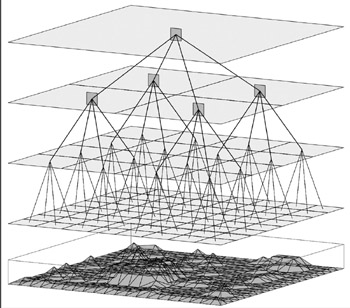
\includegraphics[width=6cm]{img/quadtree.png}
   \caption[Quadtree]{Quadtree\protect\footnotemark}
   \label{fig:quadtree-img}
 \end{wrapfigure}
 \footnotetext{Extrait de \url{https://flylib.com/books/en/2.124.1.130/1/}}
  
 Un Quadtree est une structure de données s'apparentant à un arbre ou chaque noeud de l'arbre possède quatre fils. Utiliser un Quadtreee est un bon moyen de diviser un terrain en plusieurs région. On peux ainsi représenter un terrain en deux dimensions en le divisant en quatre plus petites régions égaux, puis chaque régions obtenues en quatre sous-régions, et ainsi de suite, avec chaque noeud comprenant des données correspondant à une sous-région. Pour à terme obtenir la région initial divisé en \begin{math}{4^n}\end{math} plus petite région de même taille avec n la hauteur de l'arbre.

  
\vspace{1.5cm}
  \section{Chuncked LOD}
  
  La méthode \textbf{CDLOD}, est basé sur la méthode \textbf{CLOD} "Chuncked LOD" développé par Thatcher Ulrich~\cite{CLOD}.
  Afin de mieux comprendre la CDLOD il est donc nécessaire de présenter la méthode CLOD.

\begin{figure}[!ht]
    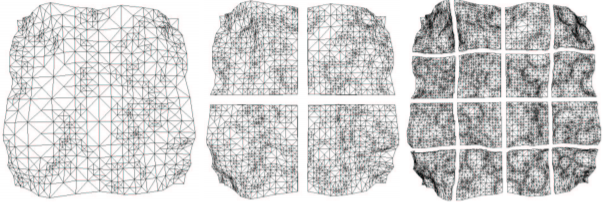
\includegraphics[width=12cm]{img/clod.png}
    \caption[CLOD]{CLOD\protect\footnotemark}
    \label{fig:clod}
\end{figure}
\footnotetext{Extrait de \url{http://tulrich.com/geekstuff/sig-notes.pdf}}


  La méthode CLOD utilise un \textbf{Quadtree} afin de stocker les différents "Level Of Detail". Dans un premier temps il est nécessaire de stocker au préalable les niveaux de détails dans le Quadtree. Lors de l'exécution , les LOD nécessaire sont calculé et ainsi utilisé depuis le Quadtree. 
  
  Pour appliqué une texture il suffit alors d'associer chaque "chunck" (noeud) à une texture.
  Le rendue du terrain est alors fait en fonction de la distance par rapport ç la caméra. C'est à dire que les noeud sont sélectionné pour être en fidèle au terrain. Pour ce faire à chaque noeud du Quadtree est associé une erreur maximal et un volume englobant tel que :
  
  {\Large
\begin{center}
  \begin{math}
  p=\frac{\delta}{D}K
  \end{math}
 \end{center}
 }
 
 \begin{itemize}
\item \emph{p} : erreur de l'espace maximale de ce noeud;
\item \begin{math}\delta\end{math} : erreur géométrique maximale associé au bloc;
\item D : distance entre la caméra et le point le plus proche sur le bloc.
\item K : facteur d'échelle en perspective qui prend la taille de la fenêtre et le champ de vision en considération
\end{itemize}
  
  K est obtenue de tel manière: 

  {\Large
\begin{center}
  \begin{math}
  K=\frac{tailledelafenetre}{2*tan\frac{champdevision}{2}}
  \end{math}
 \end{center}
 }
 
 Pour affiché un noeud, le Quadtree est parcourue depuis la racine avec \emph{p} de tolérance maximum prédéfinie. Si le \emph{p} du noeud parcourue est valide il est affiché et si il y a un trop grand écart alors on continue dans ses fils du Quadtree, et ainsi de suite.
 
 Lorsqu'un noeud est sur le point d'être réduit à ses fils ou inversement ses fils regroupé en sont parents , il va alors se produire un effet "flash"/une apparition brusque de la grille. La méthode résout se problème en ajoutant un petit "morphing" (une transition fluide). Pour se faire la méthode consiste à ajouter un point et de le décaler de tel sorte que cela corresponde eu niveau de détail souhaiter(plus grand ou plus petit)
 
 
 \begin{figure}[!ht]
    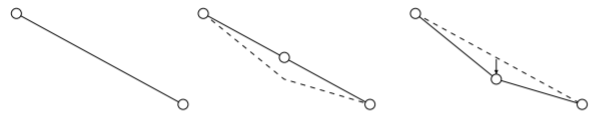
\includegraphics[width=12cm]{img/morph.png}
    \caption[morph]{ Illustration \protect\footnotemark}
    \label{fig:morph-pop}
\end{figure}
\footnotetext{Extrait de \url{http://tulrich.com/geekstuff/sig-notes.pdf}}

Dans cet exemple la ligne de gauche est composé de deux sommets, on va ensuite venir y ajouter un troisième sommet (ligne du milieu) pour augmenter le niveau de détail, que l'on va par la suite faire glisser afin que cela corresponde bien au niveau de détail augmenté.

Un nouveau problème va donc par la suite apparaître. Comme expliqué plus haut la différence entre deux niveaux de détails voisins va faire apparaître des discontinuité. Ulritch.T pour se faire va alors en quelque sorte "remplir" ces trous en créant un "rideau" composé de la même texture dont il va se servir pour combler le vide entre les noeuds.

 \begin{figure}[!ht]
    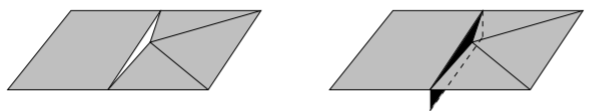
\includegraphics[width=12cm]{img/skirt.png}
    \caption[morph]{ Résolution du problème de discontinuité \protect\footnotemark}
    \label{fig:skirt}
\end{figure}
\footnotetext{Extrait de \url{http://tulrich.com/geekstuff/sig-notes.pdf}}

Le problème de cette méthode est que pour s'assurer que le "rideau" couvre la totalité de la zone vide, il doit partir du sommet le plus haut de la zone et le faire descendre à la vertical en dessous de la totalité du niveau de détail. C'est à dire peut-être(et même dans la plus part du temps) au dessous du niveau actuel(Comme on peux le voir sur la figure ci-dessus).

\section{Continuous Distant-Dependent LOD}

Comme énoncé précédemment la méthode CDLOD de Filip Strugar est basé sur CLOD, mais diffère en de nombreux points que nous allons abordé.
L'algorithme s'organise également autour de la Heightmap stockée dans un Quadtree est va assuré que le nombre de triangles affiché à l'écran soient constant, quelle que soit la distance de la caméra.

\subsection{Transitions de LOD}
    l'algorithme de CDLOD garde en continue un niveau de détail en utilisant sans arrét des transitions. Contrairement à la méthode Chuncked-LOD de Ulrich.T ~\cite{CLOD} , Strugar.F dans sa méthode ~\cite{CDLOD}, n'utilise pas de "rideau" pour combler le vide provoqué par la différence de niveau de détail, mais s'assure que le maillage du niveau supérieur soit complétement transformé en maillage de niveau inférieur avant que la changement ne se produise. Cela signifie qu'il n'y aura aucune apparition brusque,ni de discontinuité.
    
\begin{figure}[!ht]
    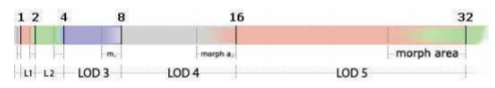
\includegraphics[width=12cm]{img/morph-area.png}
    \caption[morph-area]{Zone de transition \protect\footnotemark}
    \label{fig:morph-area}
\end{figure}
    \footnotetext{Extrait de \url{http://www.vertexasylum.com/downloads/cdlod/cdlod_latest.pdf}}
    
    La zone de transition couvre environ 15 à 30\% de chaque LOD,
    
\subsection{Implémentation de la Transition}

  L'opération de "morphing" est fait dans le vertex shader et chaque noeud peut être transformé pour correspondre à un noeud, soit un niveau plus élevé ou un niveau inférieur dans la quadtree. La morph est réalisée de telle manière que chaque bloc de 8 triangles sont  facilement transformé en un bloc correspondant de 2 triangles. Ce morphing se traduira par des transitions en douceur sans discontinuité.
  Lors du rapprochement(ou éloignement) de la caméra les sommets sont déplacé verticalement pour correspondre au niveau souhaité (voir ci-dessous).
\begin{figure}[!ht]
    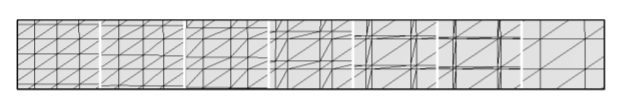
\includegraphics[width=12cm]{img/morph-transition.png}
    \caption[morph-transition]{Représentation des transitions \protect\footnotemark}
    \label{fig:morph-transition}
    \end{figure}
    \footnotetext{Extrait de \url{http://www.vertexasylum.com/downloads/cdlod/cdlod_latest.pdf}}
    
\subsection{Sélection de LOD}
    
    La méthode de sélection est le même que pour CLOD hormis sur certains points. En effet, La méthode CLOD se base pour la sélection de LOD sur de la distance sur une dimension 2D sans tenir compte de la hauteur. Strugar.F quant à lui se place dans un environnement en 3 dimension en faisant une approximation de la distance (hauteur comprise) basé sur la LOD.


\subsection{Basic et Streaming Version}

    Il existe deux façons de stocker le Quadtree qui d'une version à l'autre réduit considérablement la mémoire utilisé. En effet la version BasicCDLOD assez simple à mettre en oeuvre étend et stock entièrement tout les LOD, et, va venir parcourir la structure de donnée afin de sélectionné les niveaux nécessaire.
   
    Une autre version proposé, plus complexe à mettre en oeuvre mais qui économise grandement la mémoire, est la méthode StreamingCDLOD où seuls les parties nécessaires à la vue actuelle sont conservés. Les noeuds sont ensuite permutées si nécessaire. Par conséquent, les noeuds qui n'ont pas été utilisé pendant un certain temps peuvent être libérés.